\section{Data Presentation}
Firstly, some exploratory data analysis will be performed in order to check whether or not the S\&P-500 returns satisfy the stylized facts of financial time series as described in Section \ref{fedpik}. We recall the basic stylized facts of financial time series as the following:
\begin{enumerate}
    \item Volatility clustering.
    \item No significant autocorrelation in the log-returns $R=(R_{t})_{t\in\Z}$.
    \item Significant autocorrelation in $(|R_{t}|)_{t\in \Z}$ and $(R_{t}^{2})_{t\in \Z}$.
    \item The emperical distribution of $R$ is leptokurtic. 
    \item The leverage effect.
\end{enumerate}
Our emperical data is the daily closing value of the S\&P-500 index from \textcolor{red}{2000-01-03 to 2021-12-10}. The total number of observations is 5522, and thus the total number of observations in the log-returns time series $R$ is 5521. A plot of the raw data looks as follows: 
\begin{figure}[H]
    \centering
    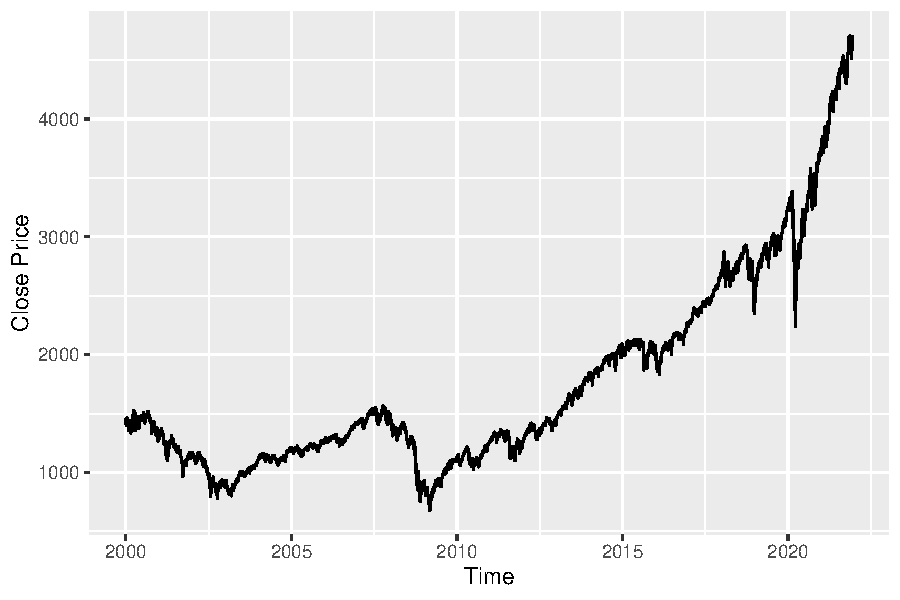
\includegraphics[scale=0.7]{fig/img/rawplotny.pdf}
    \caption{Daily Closing Value of S\&P-500 Index from 2000-01-30 to 2021-12-10.}
    \label{fig:rawplot}
\end{figure}
Clearly, this is a non-stationary time series with an upward trend abrupted by some periods with a spike in volatility. Testing the null hypothesis of non-stationary of the time series using the augmented Dickey-Fuller test yields a p-value of 0.99, which clearly exceeds any reasonable significance level. Furthermore, plotting the process of log-returns $(R_{t})_{t=1}^{5521}$ clearly supports the first stylized fact of volatility clustering: 
\begin{figure}[H]\label{volahej}
    \centering
    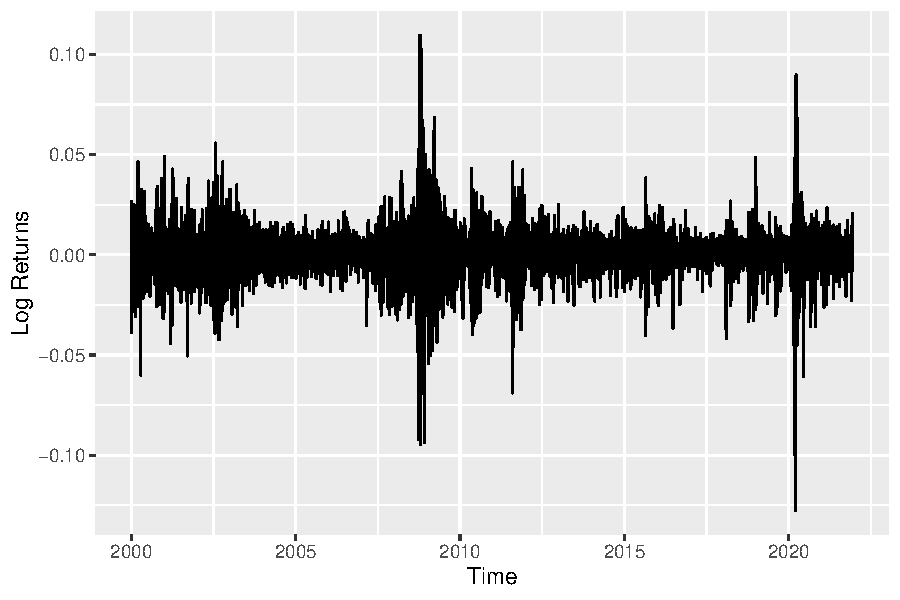
\includegraphics[scale=0.7]{fig/img/log-return-ny.pdf}
    \caption{Log-Returns of the S\&P-500 Index from 2000-01-03 to 2021-12-10.}
    \label{fig:plot2}
\end{figure}
Volatility clustering is clear, especially in the time periods surrounding the financial crisis of 2008, and the emergence of COVID-19 in 2020, both of which generated a great amount of disturbance in the financial markets. Since the log-returns time series $(R_{t})_{t=1}^{5521}$ in Figure 2.2 resembles a white noise process with volatility spikes, we expect the corresponding correlogram to show no significant autocorrelation in the log-returns. Plotting the sample autocorrelation $\hat{\rho}_{R}$ along with the confidence bands of $\pm \Phi^{-1}(1-\alpha/2)/\sqrt{n}$, where $\Phi^{-1}:[0,1]\to \R$ is the quantile function of the standard normal distribution, yields Figure 2.3.
\begin{figure}[H]
    \centering
    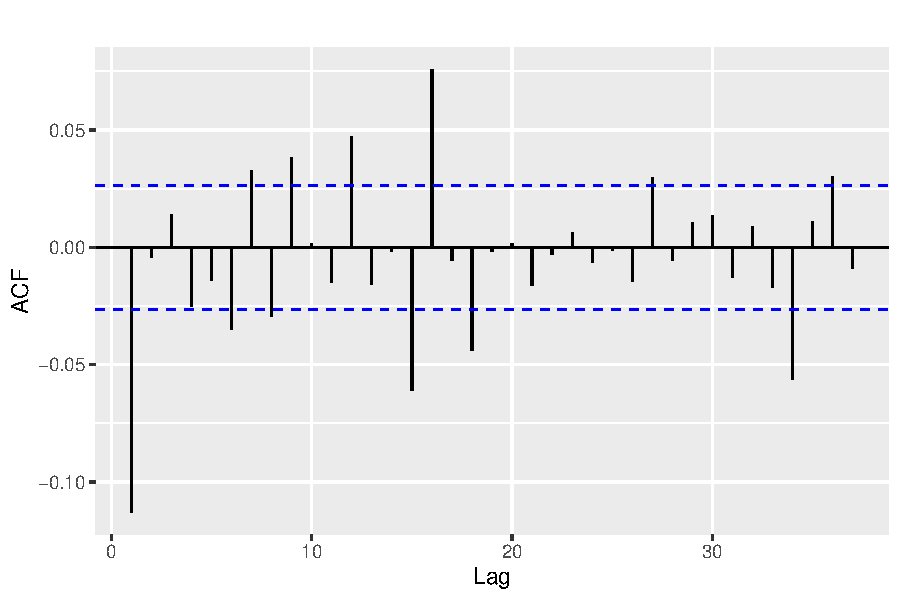
\includegraphics[scale=0.7]{fig/img/nytacfplotwuhuuu.pdf}
    \caption{Correlogram of the Log-Return Time Series.}
    \label{fig:my_label}
\end{figure}
Please note that for the given plot, we have chosen a significance level of $\alpha=0.05$ \textcolor{red}{and the number of observations is $n=5521$.} It is clear that for all lags greater than 2, there is no significant autocorrelation in the return process, since most correlations are bounded by the confidence bands with a few exceptions slightly rising above the bands. We can formally test whether these autocorrelations are significant or not using the Ljung-Box test. Testing the null hypothesis of independence on the log-returns using the Ljung-Box Q-statistic \eqref{eq:lb-qts} yields the following p-values: 
\begin{figure}[H]
    \centering
    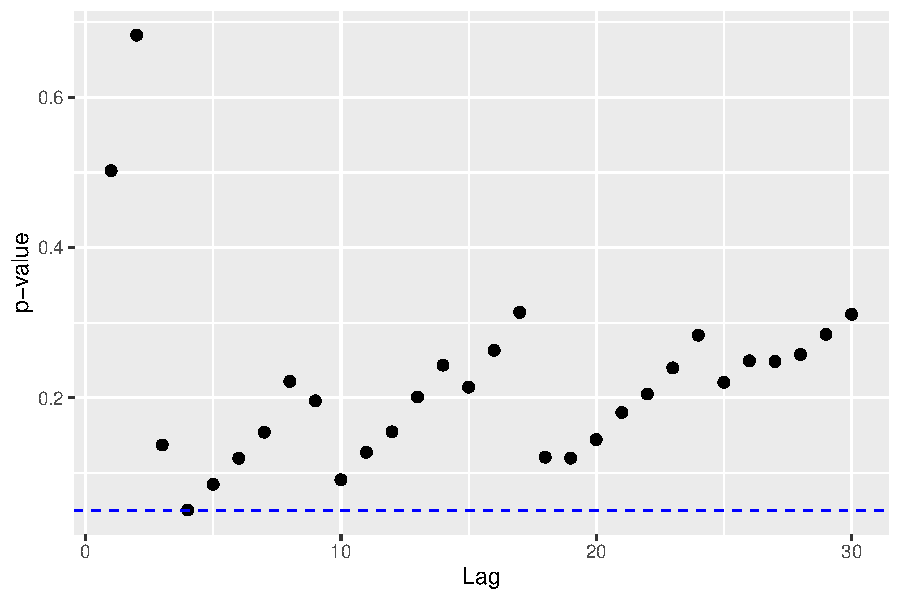
\includegraphics[scale=0.7]{fig/img/ny_ljnugbox_ggplot.pdf}
    \caption{P-values for the Ljung-Box Q-Statistic.}
    \label{fig:ljungbox}
\end{figure}
%\textcolor{red}{Det her plot er kun for de første 90 observationer af log-return serien.} 
The plot of p-values shows that at none of the first 30 lags is it possible to reject the null hypotheis of independence.
%Testing the null hypothesis of independence, and thus also whether the given ACF-values are uncorrelated, yields a p-value of 0.98. 
%This clearly exceeds any reasonable significance level, and thus we cannot reject the null hypothesis of independence.
Thus, we accept the log-returns as being independent, and hence by implication, they are also uncorrelated. 

Proceeding accordingly, the correlogram of the processes $(|R_{t}|)_{t=1}^{5521}$ and $(R_{t}^{2})_{t=1}^{5521}$ are plotted in the following Figure 2.5 and Figure 2.6 respectively:
\begin{figure}[H]
\begin{minipage}[b]{0.45\linewidth}
\centering
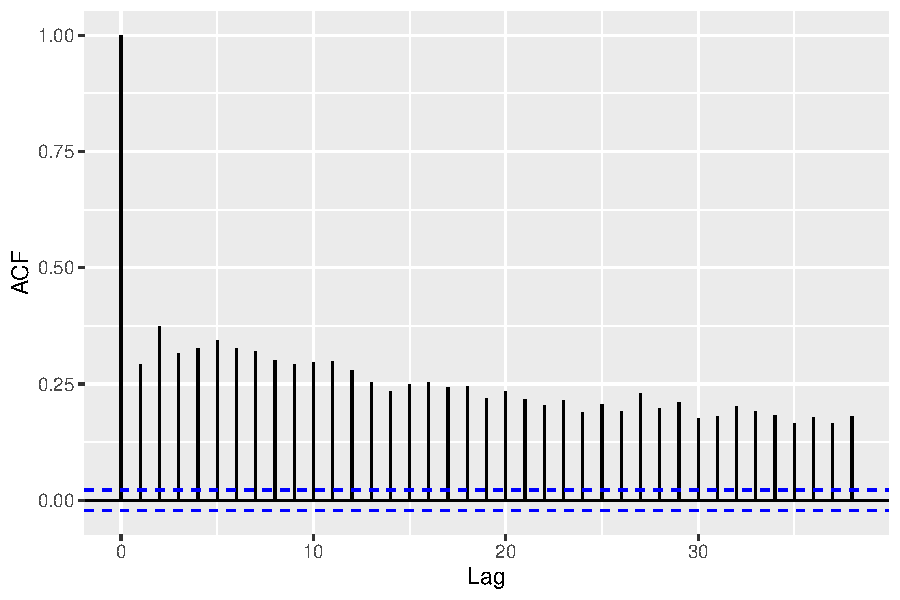
\includegraphics[width=1.2\linewidth, height=0.3\textheight]{fig/img/acfabsret.pdf}
\caption{Correlogram of $(|R_{t}|)_{t=1}^{5521}$.}
\label{fig:ACF1}
\end{minipage}
\hspace{0.7cm}
\begin{minipage}[b]{0.45\linewidth}
\centering
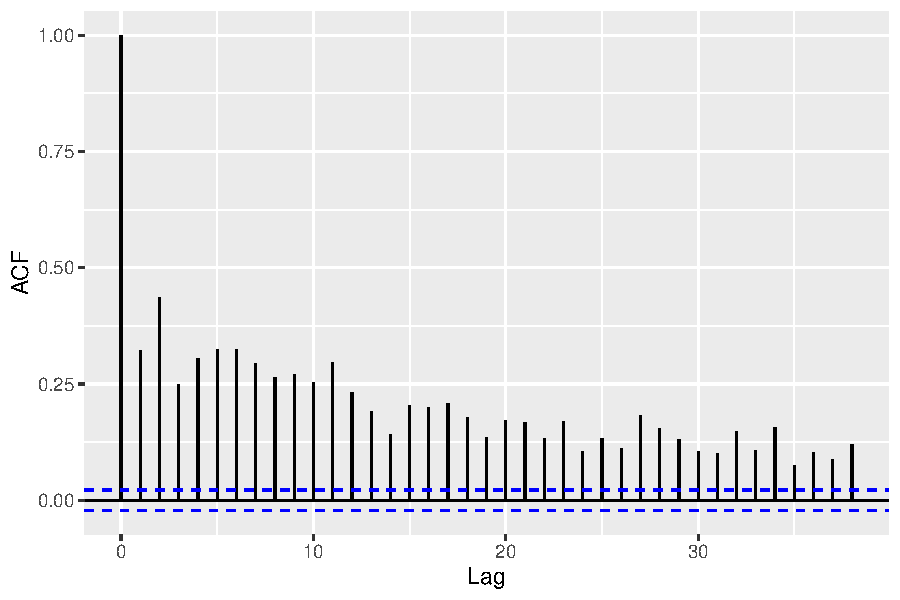
\includegraphics[width=1.2\linewidth, height=0.3\textheight]{fig/img/acfsquaredret.pdf}
\caption{Correlogram of $(R_{t}^{2})_{t=1}^{5521}$.}
\label{fig:ACF2}
\end{minipage}
\end{figure}
Evidently, there is strong autocorrelation in the processes of absolute and squared log-returns for all lags greater than 1. Thus, we now turn to the third stylized fact, which addresses whether the empirical distribution of $R$ is leptokurtic. Comparing the sample quantiles against the quantiles of a normal distribution gives the following QQ-plot:\vspace{-6 pt}
\begin{figure}[H]
    \centering
    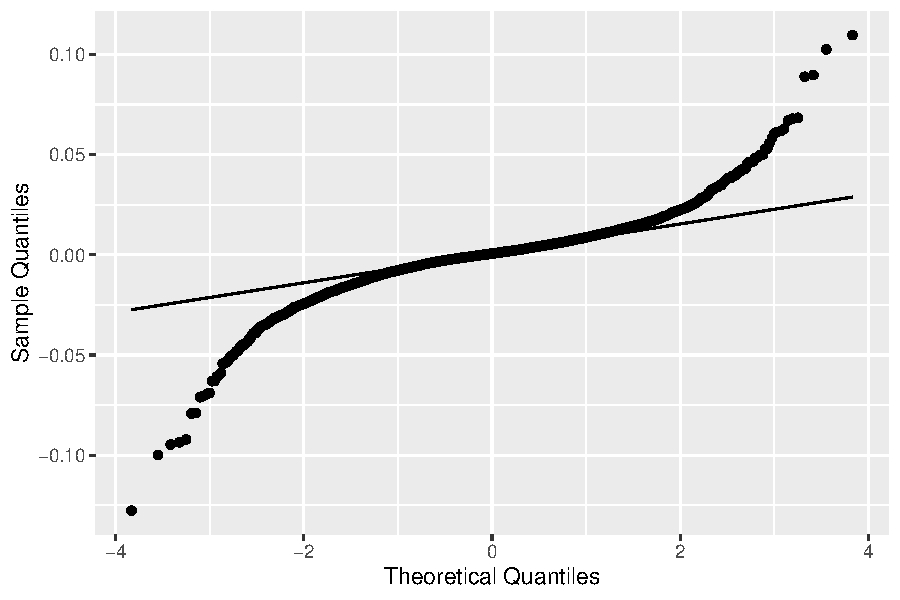
\includegraphics[scale=0.7]{fig/img/qqplot.pdf}
    \caption{QQ-Plot of Sample Quantiles against Normal Quantiles.}
    \label{fig:qqplot1}
\end{figure}
The return process is visibly much more heavy-tailed than the normal distribution with much more probability mass condensed at the tails. Furthermore, the empirical histogram $H_{R}:\R\to [0,\infty)$ of the return process $R$ with fineness of partition $k$ is then given by:
\begin{equation}
    H_{R}(x)=\frac{2^{k}}{N}\sum_{i=1}^{N}\ind_{\left(\frac{j_{k}(x)-1}{2^{k}},\frac{j_{k}(x)}{2^{k}}\right]}(R_{i}),
\end{equation}
where $N$ is the number of observations in our return process, and $j_{k}(x)\coloneqq [2^{k}x]$ for $x\in \R$. We can plot this function $H_{R}$ along with the normal density $f\sim \mathcal{N}(\mu,\sigma^{2})$, where the parameter $\mu$ is chosen as the mean of the return process, and $\sigma$ is similarly the standard deviation of the return process. Additionally, the non-parametric kernel density estimate of the return process is drawn in blue. The resulting plot is then:
\begin{figure}[H]
    \centering
    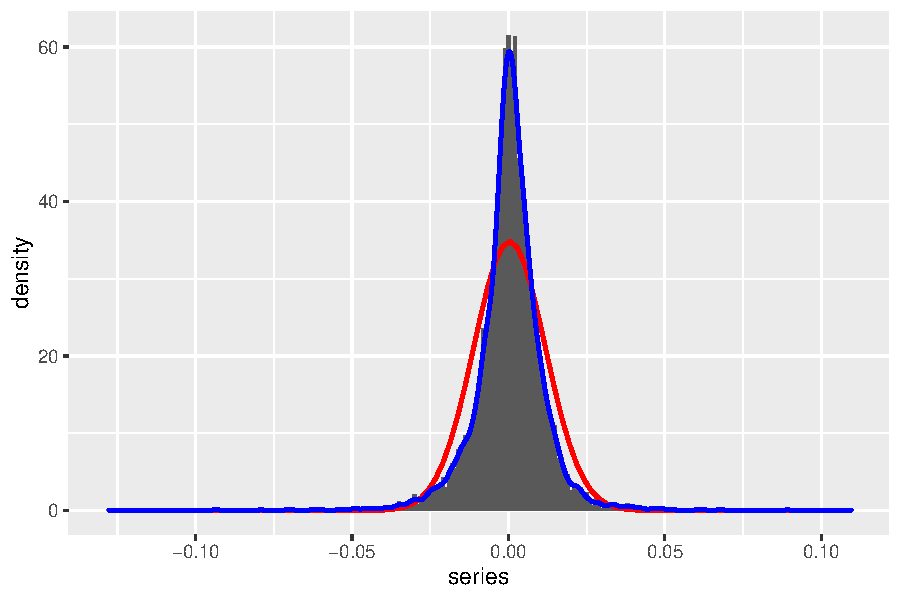
\includegraphics[scale=0.75]{fig/img/histogramplot.pdf}
    \caption{Empirical Histogram with Theoretical Normal Density and Estimated Density.}
    \label{fig:my_label}
\end{figure}
Evidently, the empirical distribution of the log-returns is more sharply spiked at the center than the corresponding normal density drawn in red. Similarly, the kernel density decays more slowly than exponentially, indicating that the empirical distribution is leptokurtic. Calculating the sample kurtosis of the log-returns series confirms this, yielding a kurtosis coefficient of 14.07, which is significantly above the mesokurtic level of 3.

Turning to the final stylized fact concerning the leverage effect, we can check how the time series $R^{+}_{t}\coloneqq \max\{ R_{t},0\}$ and $R^{-}_{t}\coloneqq \min\{-R_{t},0\}$ are correlated with the absolute returns $|R_{t}|$. As indicated by Figure 2.9, there is strong cross-correlation between $|R_{t}|$ and $R^{+}_{t}$ with all lags rising above the confidence bands. However, there is even stronger cross-correlation between $|R_{t}|$ and $R^{-}_{t}$, especially for positive lags, which rise significantly above $0.2$. Hence, Figure 2.10 supports the presence of the leverage effect in the data, indicating that market volatility increases more, when returns are negative.
%The observations of $|R_{t}|$ and $R^{+}_{t}$ are approximately 54\% equal and conversely, we have that the observations of $|R_{t}|$ and $R^{-}_{t}$ are approximately 46\% equal.
\begin{figure}[H]
\begin{minipage}[b]{0.45\linewidth}
\centering
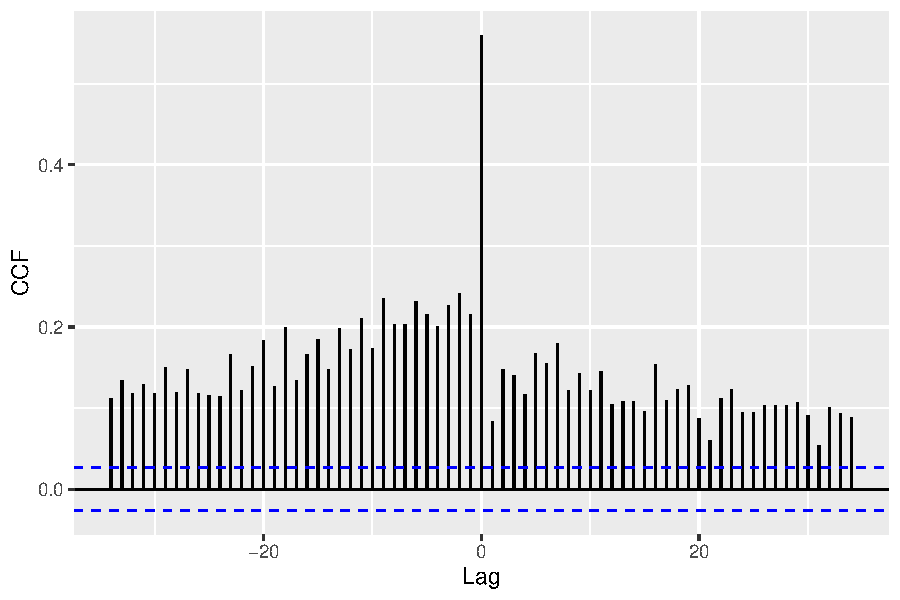
\includegraphics[width=1.2\linewidth, height=0.3\textheight]{fig/img/ccfmaxRny.pdf}
\caption{CCF of $|R_{t}|$ and $R^{+}_{t}$.}
\label{fig:ACF1}
\end{minipage}
\hspace{0.7cm}
\begin{minipage}[b]{0.45\linewidth}
\centering
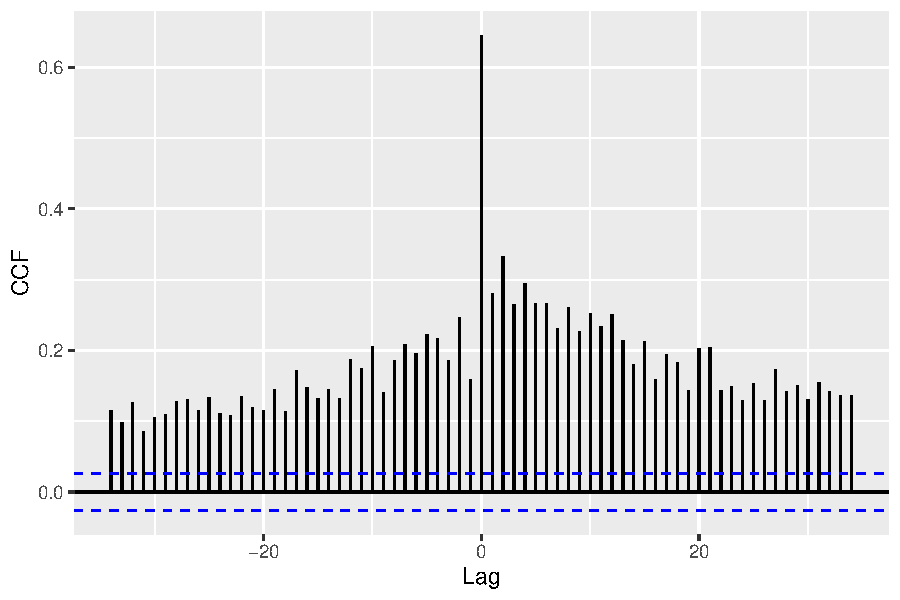
\includegraphics[width=1.2\linewidth, height=0.3\textheight]{fig/img/ccfminusR.pdf}
\caption{CCF of $|R_{t}|$ and $R^{-}_{t}$.}
\label{fig:ACF2}
\end{minipage}
\end{figure}
Generally, the cross-correlations are numerically large for both negative and positive lags, signifying that either series leads or lags the other. This comes as no surprise, since the two series have a vast overlap of observations. Approximately 54\% of the observations in $|R_{t}|$ and $R^{+}_{t}$ are equal, and conversely, we have that approximately 46\% of the observations in $|R_{t}|$ and $R^{-}_{t}$ are equal. 

\begin{table}[H]
\centering
\begin{tabular}{llllllll}
\hline
$h$ & 1 & 2 & 3 & 4 & 5 & 6 & 7 \\ \hline
$\hat{\rho}_{R}(h)$ & -0.1128 & -0.0043 & 0.0139 & -0.0252 & -0.0139 & -0.0351 & 0.0326 \\
$\hat{\rho}_{|R|}(h)$ & 0.3078 & 0.4033 & 0.3395 & 0.3458 & 0.3616 & 0.3523 & 0.3412\\
$\hat{\rho}\left(R^{+}_{t-h},|R_{t}|\right)$ & 0.0839 & 0.1473 & 0.1404 & 0.1164 & 0.1675 & 0.1554 & 0.1791\\ 
$\hat{\rho}\left(R^{-}_{t-h},|R_{t}|\right)$ & 0.2801 & 0.3326 & 0.2649 & 0.2942 & 0.2655 & 0.2659 & 0.2311 \\ \hline
\end{tabular}
\end{table}
%Specifically, it will be checked if the empirical distribution of log-returns is leptokurtic, if there is significant autocorrelation in absolute log-returns, and if there is significant autocorrelation in squared log-returns. The dataset to be utilized is the S\&P-500 index. We have chosen the daily closing value of the index in the time span 2006-MM-DD to 2021-MM-DD.

%The results of the
